\pdfminorversion=4
\documentclass[aspectratio=169]{beamer}

\mode<presentation>
{
  \usetheme{default}
  \usecolortheme{default}
  \usefonttheme{default}
  \setbeamertemplate{navigation symbols}{}
  \setbeamertemplate{caption}[numbered]
  \setbeamertemplate{footline}[frame number]  % or "page number"
  \setbeamercolor{frametitle}{fg=white}
  \setbeamercolor{footline}{fg=black}
} 

\usepackage[english]{babel}
\usepackage{inputenc}
\usepackage{tikz}
\usepackage{courier}
\usepackage{array}
\usepackage{bold-extra}
\usepackage{minted}
\usepackage[thicklines]{cancel}
\usepackage{fancyvrb}

\xdefinecolor{dianablue}{rgb}{0.18,0.24,0.31}
\xdefinecolor{darkblue}{rgb}{0.1,0.1,0.7}
\xdefinecolor{darkgreen}{rgb}{0,0.5,0}
\xdefinecolor{darkgrey}{rgb}{0.35,0.35,0.35}
\xdefinecolor{darkorange}{rgb}{0.8,0.5,0}
\xdefinecolor{darkred}{rgb}{0.7,0,0}
\definecolor{darkgreen}{rgb}{0,0.6,0}
\definecolor{mauve}{rgb}{0.58,0,0.82}

\title[2024-01-10-compute-accelerator-garbage-collectors]{Three garbage collectors: Java, Python, and Julia}
\author{Jim Pivarski}
\institute{Princeton University -- IRIS-HEP}
\date{January 10, 2024}

\usetikzlibrary{shapes.callouts}

\begin{document}

\logo{\pgfputat{\pgfxy(0.11, 7.4)}{\pgfbox[right,base]{\tikz{\filldraw[fill=dianablue, draw=none] (0 cm, 0 cm) rectangle (50 cm, 1 cm);}\mbox{\hspace{-8 cm}
\includegraphics[height=1 cm]{princeton-logo-long.png}\hspace{0.1 cm}\raisebox{0.1 cm}{
\includegraphics[height=0.8 cm]{iris-hep-logo-long.png}}\hspace{0.1 cm}}}}}

\begin{frame}
  \titlepage
\end{frame}

\logo{\pgfputat{\pgfxy(0.11, 7.4)}{\pgfbox[right,base]{\tikz{\filldraw[fill=dianablue, draw=none] (0 cm, 0 cm) rectangle (50 cm, 1 cm);}\mbox{\hspace{-8 cm}
\includegraphics[height=1 cm]{princeton-logo.png}\hspace{0.1 cm}\raisebox{0.1 cm}{
\includegraphics[height=0.8 cm]{iris-hep-logo.png}}\hspace{0.1 cm}}}}}

% Uncomment these lines for an automatically generated outline.
%\begin{frame}{Outline}
%  \tableofcontents
%\end{frame}

% START START START START START START START START START START START START START

\begin{frame}{Dynamic language/programming features}
\vspace{0.2 cm}
\begin{center}
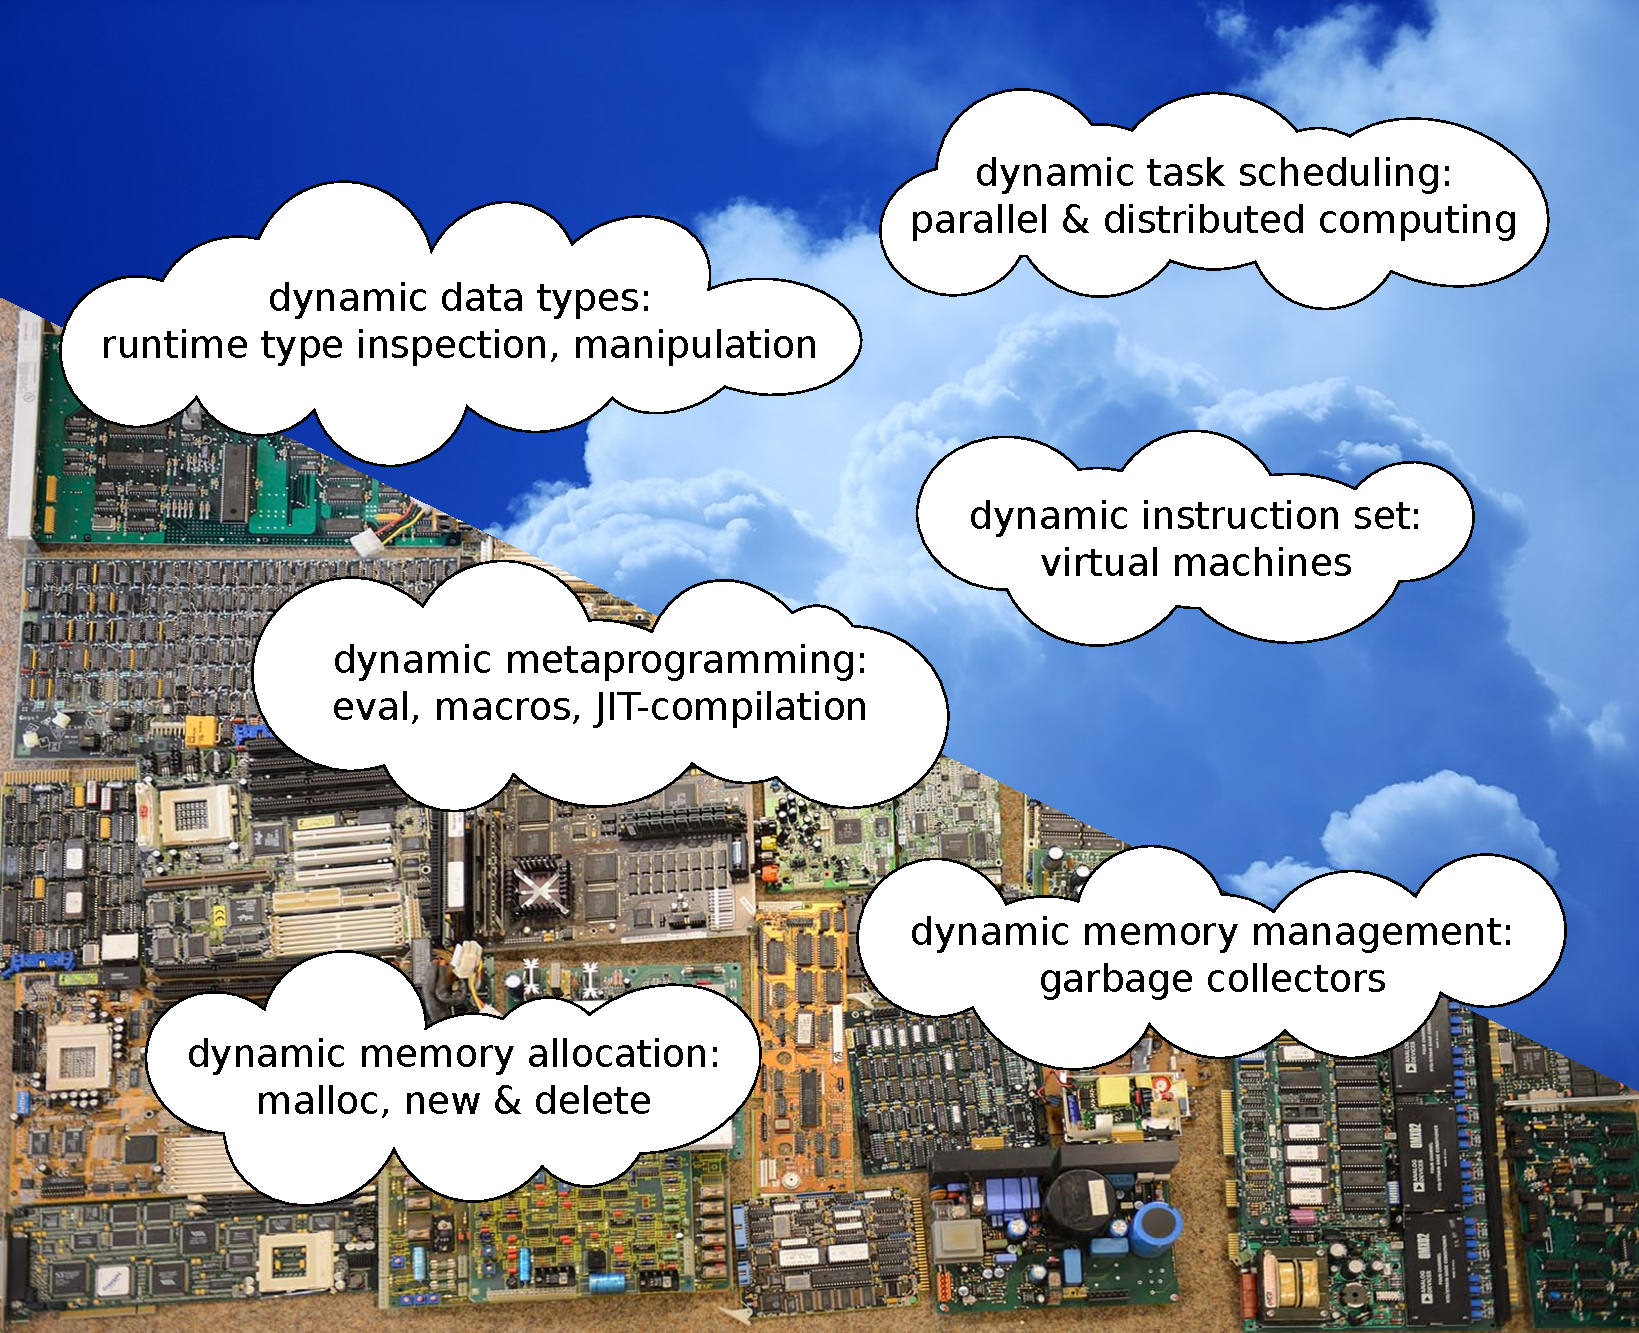
\includegraphics[width=0.67\linewidth]{dynamic-features.pdf}
\end{center}
\end{frame}





\end{document}

%% Yes, I've run into performance problems with garbage collectors in previous projects, though they were particular situations that can perhaps be avoided.

%% Specifically, I was working in Java, developing a distributed pipeline. When one step passed data along to another step, it would go into the latter's input queue. The problem was that this JVM would occasionally pause for garbage collection, and during that time, its input queue filled up. With a lot more (garbage collectable) objects in the input queue, it would have more garbage collection to do, and the situation spiraled out of control—it was a positive feedback loop. It was too late to re-architect the whole workflow, so I switched Java's default garbage collector for a pauseless one and tuned it until we had a working system if it stayed within certain parameters.

%% That's a more specific problem than just having long-running jobs. I can't think of any particular issue with long-running jobs and garbage collectors—it's not unusual for Python processes to be long-running.

%% Another issue with garbage collectors (more recent Python experience) is that they make memory performance harder to debug. Often, Uproot users report memory leaks when they see memory use increase linearly in a loop, but then when I investigate, it turns out that the garbage collector just hadn't decided to trigger yet. When it does, the memory use becomes flat. (This isn't always the case: users have reported real, significant memory leaks. It's just harder to debug because sometimes it's a mismatch between their assumption that the memory will be released immediately when in fact the collector just hasn't triggered yet.)

%% On this point, an important question is, "what triggers garbage collection?" That's something I've been intending to understand better. I had previously thought that Linux processes knew how much memory is available and would trigger garbage collection when, say, they've reached the 90% limit. I've done some experiments putting processes in a memory-limited box like

%% systemd-run --user --scope -p MemoryMax=100M -p MemorySwapMax=0M python ...

%% and I see that they trigger garbage collection earlier, to stay within the box. But Enrico Guiraud told me that Linux has no such mechanism, so I'm going to need to do some reading and more experiments to be sure.

%% Summary of three garbage collectors:
%% Java: 
%% compactifies (copies) data in generational buckets, so all references are pointers-to-pointers (pointer chasing)
%% many options, and the default has changed through the years
%% old default would "stop the world," which was my problem with the distributed workflow; new default from Java 15 onward is pauseless
%% Python: 
%% reference counting is the primary collector (in CPython, not PyPy), so data without reference cycles should get freed immediately after going out of scope; reference counters use a lot of memory, though
%% uses a number of allocations (in three generations) since last collection to decide when to trigger (reference, I just found this), then it's a stop-the-world mark-and-sweep
%% allocates data into its own arenas, so the memory use reported to the operating system can be more than what Python is actually using; that could explain some of the spurious memory leak reports
%% Julia: 
%% summary from the documentation; summary from Stefan Karpinsk
%% no compactification and no reference counters: all garbage collector information is encoded in two bits of tagged pointers, one for the mark-and-sweep mark, and another for age (so exactly two generations, then)
%% Julia's pool allocation of small objects sounds to me like the private arenas that complicate Python memory debugging, but the same page says that it malloc's arrays and large objects, so it might not matter (you only need to debug large memory issues)
%% this comment from Sep 2021 leads me to believe that Julia's garbage collector is single-threaded and stops the world: "That’s basically how I can see the GC pauses: when the computation only eats 1 CPU as seen in htop." This StackOverflow answer would confirm it, but it's 8 years old. Do you have more recent information on these two aspects of Julia's garbage collector, is it multithreaded and does it pause execution?
%% I also don't know if it's possible to tune Julia's garbage collector nowadays
%% instead of exclusively relying on the garbage collector, as Java and Python mostly* do, Julia tries to get as many objects as possible on the stack, rather than the heap. Immutable data structures are preferred in order to encourage this (tutorial, HackerNews). I had thought there was a way to force Julia objects onto the stack with a macro, but I couldn't find it on the Performance Hints page. Anyway, stack allocation (and performance in general) is a more frequent topic of discussion in Julia circles than in Java and Python.
%% * Java and Python have internal optimizations to use the stack when escape analysis says it's possible, but less aggressively than Julia.

%% So, just being a long-running process doesn't sound to me like a reason to avoid garbage collectors, but I don't know the rest of the context. In fact, the memory safety that garbage collectors (or Rust) provide sounds important for a long-running process: the probability of mistakes in manual memory management is compounded by time.

%% I had particular issues with a stop-the-world garbage collector in the past, but that situation can be avoided with workflow design, once you know that it can be an issue.

%% Finally, a language is not just the technical details of its implementation; it's also a community that has certain priorities. The Julia community is obsessed with performance, so it's easy to get help about performance issues (and hard to avoid getting performance hints when your question is not performance related...). If it's really true that the Julia garbage collector is still single-threaded, stop-the-world, I'd be surprised, but there would also be a lot of motivation in the community to fix it or at least point out ways to avoid heap-allocation.
